\section{Wyniki}
Pomimo stosunkowo krótkiego działania skanera, udało zaobserwować się, że wiele domen rzeczywiście odpowiada na zapytania AXFR. Konkretne wyniki zostały zaprezentowane na rysunku \ref{fig:odpowiedzi}. Możemy zauważyć, że w kilku iteracjach było bardo wiele odpowiedzi. Dane wejściowe były uporządkowane według nazw, więc można postawić hipotezę, że o te same domeny odpytywano kilka serwerów autorytatywnych i większość była rzeczywiście źle skonfigurowana. Innym powodem może byc po prostu czynnik losowy, jednak zastanawiające jest, że trzy iteracje znacznie wyróżniają się na tle innych.


\begin{figure}
    \centering
        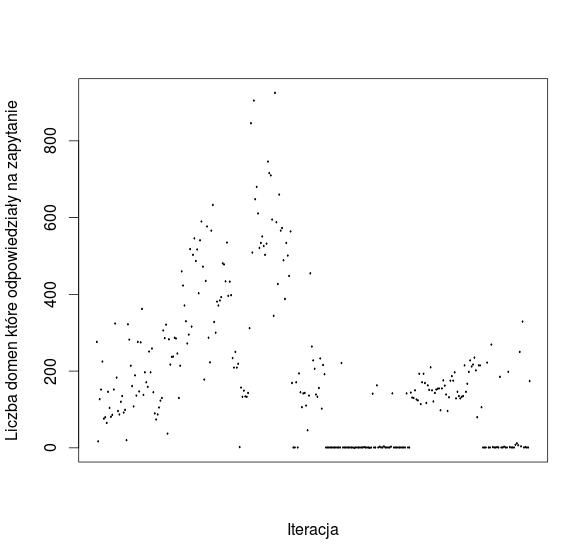
\includegraphics[width=0.8\textwidth]{odpowiedzi.png}
    \caption{ Liczba domen które odpowiedziały na zapytanie AXFR w danej iteracji.} \label{fig:odpowiedzi}
\end{figure}


Innym interesującym zjawiskiem są wpisy TXT\cite{RFC1035}, które zwracają niektóre serwery. Wpis TXT był wprowadzony głównie po to, aby ułatwić ludzie mogli przeczytać informację, która zostanie zawarta w odpowiedzi DNS. Z czasem oczywiście okazało się, że wpis częściej jest używany przez komputery niż ludzi, czego przykład mamy w odpowiedziach.

Pierwszym przykładem może być znalezienie reguły SPF\cite{RFC7208}:
\begin{lstlisting}
"v=spf1 ip4:52.72.252.186/13 ip4:52.220.30.76/15 ip4:54.179.130.187/15 ip4:52.95.240.219/20 ip4:54.251.128.33/12 ip4:114.134.29.0/23 ip4:54.169.107.198/15 ip4:46.51.216.57/20 ip4:103.228.178.81/15 ip4:157.119.230.135/14 ip4:103.44.71.16/15 ~all"
\end{lstlisting}

Z wyżej przytoczonej reguły można wywnioskować maszyny o jakich adresach są ,,specjalnie'' traktowane przez serwer. W skrócie, reguły SPF mówią, które z serwerów są upoważnione do wysyłania wiadomości z domeny. Dodatkowo parametr ,,\~all'' (jak na przykładzie powyżej) określa, że wiadomości od serwerów nie spełniających reguły będą odrzucane, lub oznaczane jako spam.

Oprócz opisanego przypadku użycia pola TXT pojawiały się także i inne, jednak nie do końca udało się je rozszyfrować. Niektóre z przytoczonych sposobów wykorzystania tego pola są oczywiście poprawne. Jednym z przykładów użycia jest wklejenie klucza publicznego. Jest to również swego rodzaju zabezpieczenie serwera przed spamem. Przykład poniżej.

\begin{lstlisting}
"v=DKIM1; k=rsa; p=MIIBIjANBgkqhkiG9w0BAQEFAAOCAQ8AMIIBCgKCAQEApt/kMkRxGXbIuiVb4lCYeTQMEOBKTXTUJya8aY659OB0feNIoA070AHq4M7/KKa4u/T/BfLNVNfyaK56S1E7S9o" "HItQUFO5idWKBRAK/VnK0I9FjWMlAMamQItiLmaUWtC4VhB5n0JzgPmutqx4qDo/IVIp97bWm3FDe4ts1zMNODxTTql52hkZ/X91/HrZYrC3qBLAg4rHbgBnJHWny55yt7vkgknyh7MAuN5qZDlN4s" "xrlOTbuJYGOCo2OTR8WteWorDC4qw41CTr273QiB/suVSZODeZD9xNKN6fmoFNCfhwUqXVzAiDVT0RcfNDmM1istoJyoVu56CCuHIJnowIDAQAB"
\end{lstlisting}

Mimo, że wpis ten wydaje się być poprawny, a nawet uzasadnione jest jego użycie, mam pewne obawy co do tego, czy rzeczywiście powinien być zwracany przez zapytanie AXFR.